\documentclass[12pt]{scrartcl}
\usepackage[sexy]{evan}
\usepackage{graphicx,amsmath,amssymb,amsthm,amsfonts,babel}
\usepackage{tikz, tkz-euclide}
\usepackage{lipsum}
\usepackage{setspace}
\graphicspath{ {./} }
\usetikzlibrary{calc,through,intersections}
\usepackage[paperwidth=16cm, paperheight=18.2cm,margin=0.65cm]{geometry}

\colorlet{EvanRed}{Red!50!Purple}

\setstretch{1.5}

\usepackage{etoolbox}
\newcommand{\zerodisplayskips}{%
  \setlength{\abovedisplayskip}{5pt}%
  \setlength{\belowdisplayskip}{5pt}%
  \setlength{\abovedisplayshortskip}{5pt}%
  \setlength{\belowdisplayshortskip}{5pt}}
\appto{\normalsize}{\zerodisplayskips}
\appto{\small}{\zerodisplayskips}
\appto{\footnotesize}{\zerodisplayskips}
\setlength\parindent{10pt}

\title{\textcolor{Red!80}{K}\textcolor{Green!80}{T}\textcolor{Blue!70}{O}\textcolor{YellowOrange!80}{M} Februari 2022}
\author{Isian no. 4, 7, 14, 16}
\date{Official solution by Azzam L. H.}


\begin{document}
\maketitle
\pagestyle{plain}


\section{Soal}
\subsection*{\protect\textcolor{EvanRed}{\S} Nomor 4} Nayeon memiliki 8 penghapus putih. Ia lalu mewarnai setiap penghapus tersebut dengan warna biru atau merah secara acak dengan peluang yang sama. Peluang bahwa untuk setiap penghapus, mayoritas (yakni, lebih dari setengah) warna dari ketujuh penghapus lain tidak sama dengan penghapus yang dijadikan acuan adalah $\frac{a}{b}$ dengan $a$ dan $b$ adalah bilangan asli yang relatif prima, tentukan nilai $a+b$.

\subsection*{\protect\textcolor{EvanRed}{\S} Nomor 7} Carilah jumlah seluruh bilangan bulat positif terurut $a$ sehingga $b$, $\dfrac{a^3b+1}{a+1}$ dan $\dfrac{2021b-2025}{b-1}$ ketiganya merupakan bilangan bulat.

\subsection*{\protect\textcolor{EvanRed}{\S} Nomor 14} Diberikan sebuah segitiga lancip $ABC$ dengan titik-titik $D,E,F$ merupakan proyeksi titik $A,B,C$ pada $BC,CA,AB$ secara berturut-turut. Misalkan $BE$ dan $CF$ bertemu di titik $H$ serta misalkan $N$ merupakan titik tengah $AH$. Besar$\angle BAC = 60^\circ$ dan $BC=16\sqrt{3}$. Jika $M$ adalah titik tengah $BC$, dan panjang $MN = x$, tentukan nilai $x^2$.


\subsection*{\protect\textcolor{EvanRed}{\S} Nomor 16} Diketahui $a,b,c$ adalah bilangan real tak nol yang memenuhi 
\begin{align*}
    ab+2bc+4ca&=1\\
    a^2b+2c&=b^2c+a\\
    16ac^2+a^2b+2c+b &= 3b^2c+3a.
\end{align*}
Jika $S=200a^2+200b^2+200c^2$, tentukan jumlah semua nilai $S$ yang mungkin.

\section{Solusi}
\subsection{Nomor 4}
Nayeon memiliki 8 penghapus putih. Ia lalu mewarnai setiap penghapus tersebut dengan warna biru atau merah secara acak dengan peluang yang sama. Peluang bahwa untuk setiap penghapus, mayoritas (yakni, lebih dari setengah) warna dari ketujuh penghapus lain tidak sama dengan penghapus yang dijadikan acuan adalah $\frac{a}{b}$ dengan $a$ dan $b$ adalah bilangan asli yang relatif prima, tentukan nilai $a+b$.
\begin{jawaban}
Perhatikan agar keadaan soal dapat terjadi, maka haruslah ada 4 penghapus biru dan 4 penghapus merah.

Ada $2^{8} = 256$ cara mewarnai seluruh penghapus dan ada ${8 \choose 4} = 70$ cara memilih empat penghapus yang akan diwarnai biru. Maka peluang yang diminta bernilai $\frac{70}{256}=\frac{35}{128}$.

Dari sini didapat $a+b = 35+128 = \boxed{163}$.
\end{jawaban}
\begin{remark}
Soal ini terinspirasi dari salah satu soal AIME 2021. Pada dasarnya soal ini hanya memanfaatkan counting mudah, oleh karena itu ditaruh di nomor 4. Perlu pemahaman yang baik akan maksud soal untuk menjawab benar.
\end{remark}

\newpage 
\subsection{Nomor 7}  Carilah jumlah seluruh bilangan bulat positif terurut $a$ sehingga $b$, $\dfrac{a^3b+1}{a+1}$ dan $\dfrac{2021b-2025}{b-1}$ ketiganya merupakan bilangan bulat.

\begin{jawaban}
Perhatikan bahwa $$\dfrac{a^3b+1}{a+1}=\dfrac{b(a^3+1)-(b-1)}{a+1} =\dfrac{b(a^3+1)}{a+1}-\dfrac{b-1}{a+1}$$ adalah bilangan bulat. Karena $a+1 \mid a^3+1$, maka $\dfrac{b(a^3+1)}{a+1}$ adalah bilangan bulat yang menyebabkan $\dfrac{b-1}{a+1}$ bulat atau $a+1 \mid b-1$.
			
			Selanjutnya, perhatikan bahwa $$\dfrac{2021b-2025}{b-1}=\dfrac{2021(b-1)-4}{b-1}=2021-\dfrac{4}{b-1}$$ adalah bilangan bulat. Karena 2021 bilangan bulat maka menyebabkan $\dfrac{4}{b-1}$ bulat atau $b-1 \mid 4$. 
			
			Dari $a+1 \mid b-1$ dan $b-1 \mid 4$, didapatkan bahwa $a+1 \mid 4$ sehingga diperoleh $a=1$ dan $a=3$. Oleh karena itu, jumlah seluruh bilangan bulat positif $a$ yang memenuhi adalah $1+3=\boxed{4}$.
\end{jawaban}
\begin{remark}
Pada dasarnya soal ini adalah versi lebih mudah dari soal nomor 4 JBMO 2013. Ide utama dari soal ini adalah menyadari bahwa bentuk $a^3+1$ terbagi oleh $a+1$ lalu dilanjutkan dengan memanfaatkan keterbagian oleh $a+1$.
\end{remark}

\newpage
\subsection{Nomor 14}
Diberikan sebuah segitiga lancip $ABC$ dengan titik-titik $D,E,F$ merupakan proyeksi titik $A,B,C$ pada $BC,CA,AB$ secara berturut-turut. Misalkan $BE$ dan $CF$ bertemu di titik $H$ serta misalkan $N$ merupakan titik tengah $AH$. Besar$\angle BAC = 60^\circ$ dan $BC=16\sqrt{3}$. Jika $M$ adalah titik tengah $BC$, dan panjang $MN = x$, tentukan nilai $x^2$.

\begin{center}
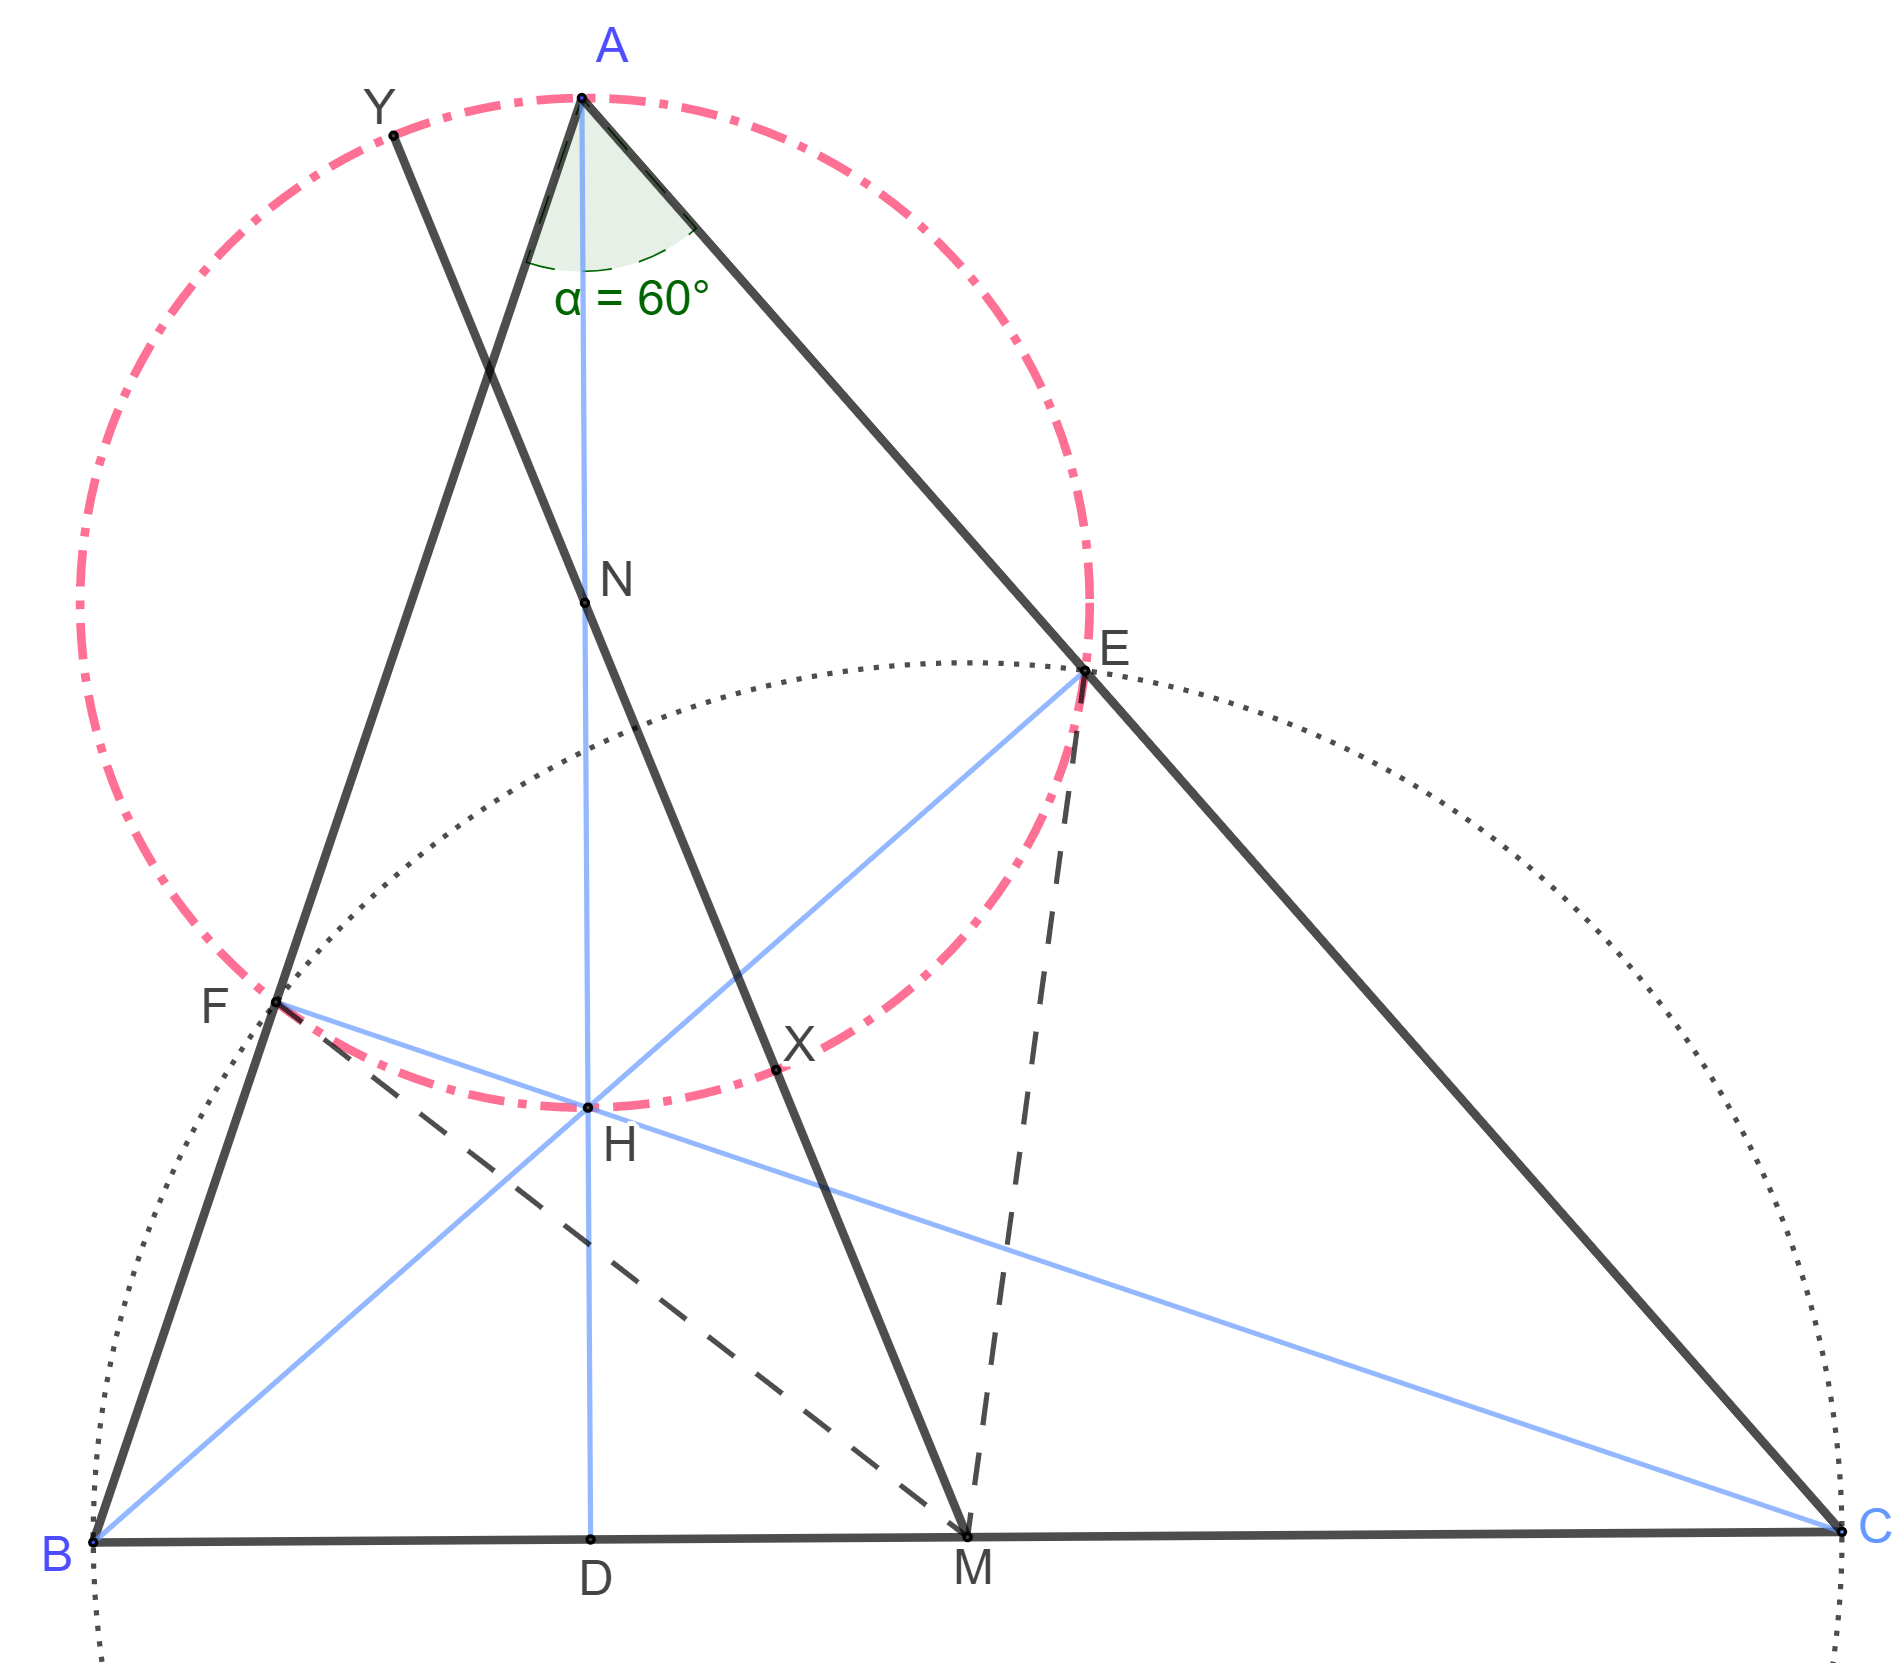
\includegraphics[scale=1.5]{nomor 14 rev.png}
\end{center}
\begin{jawaban}
Perhatikan, karena $\angle HEA = \angle HFA = 90^\circ$, maka $AEHF$ siklis dengan $N$ sebagai titik pusatnya dan $AH$ sebagai diameter. Karena $\angle BEC = \angle BFC = 90^\circ$, maka $BFEC$ siklis dengan $M$ sebagai titik pusatnya dan $BC$ diameter. 

Sekarang, karena $\angle FAC = 60^\circ$ dan $\angle AFC = 90^\circ$, maka $\angle ECF = 30^\circ$. Karena $M$ pusat lingkaran $(BFEC)$, maka $\angle EMF = 2 \angle ECF = 2 \cdot 30^\circ = 60^\circ$. Karena $EM=FM$ adalah jari-jari $(BFEC)$ dan $BC=16\sqrt{3}$ adalah diameter, maka kita menemukan $EM=FM=EF=8\sqrt{3}$.

Selanjutnya, dengan dalil Sinus di $\triangle AFE$, karena $AH$ adalah diameter lingkaran luar $\triangle AFE$, maka 
\begin{align*}
AH &= \dfrac{EF}{\sin \angle FAE}\\
AH &= \dfrac{8\sqrt{3}}{\sin 60^\circ}\\
AH &= 16
\end{align*}

Berarti lingkaran $(AEHF)$ memiliki jari-jari dengan panjang 8.

\begin{lemma}
$EM$ dan $MF$ menyinggung lingkaran $AEHF$.
\begin{proof}[Bukti Lemma]
Karena $EM=MB$ jari-jari lingkaran $(EFBC)$, maka $\angle HEM = \angle BEM = \angle EBM$. Namun, $\angle EBM = \angle EBC = \angle DAC = \angle HAE$. Itu berarti $\angle HEM= \angle HAE$ yang menunjukkan $EM$ menyinggung $(AEHF)$ di $E$. Dengan cara yang sama, dapat ditunjukkan bahwa $MF$ menyinggung $(AEHF)$ di $F$. Terbukti.
\end{proof}
\end{lemma}

Misalkan garis $MN$ memotong lingkaran $(AEHF)$ di dua titik berbeda $X$ dan $Y$, dimana $X$ berada di antara $M$ dan $N$. 

Karena $XY$ melewati $N$, maka $XY$ adalah diameter lingkaran $(AEHF)$. Oleh karena itu, dengan \textit{Power of a point}, kita punya
\begin{align*}
ME^2 &= MX \cdot MY\\
ME^2 &= MX \cdot (MX + XY)\\
(8\sqrt{3})^2 &= MX \cdot (MX + 16)\\
0 &= MX^2 + 16\cdot MX - 192\\
0 &= (MX-8)(MX+16)\\
MX &= 8\\
MN &= MX + XN\\
MN &= 8 + 8\\
MN &= 16
\end{align*}
Berarti $x=16$ dan $x^2=$\boxed{256}.

\end{jawaban}
\begin{remark}
Saya terinspirasi (dan sangat dipengaruhi) oleh Lemma 1.44 dari buku EGMO nya Evan Chen. Motivasi solusinya? Gambar yang bagus, dan baca Evan Chen :)
\end{remark}

\newpage
\subsection{Nomor 16}
Diketahui $a,b,c$ adalah bilangan real tak nol yang memenuhi 
\begin{align*}
    ab+2bc+4ca&=1\\
    a^2b+2c&=b^2c+a\\
    16ac^2+a^2b+2c+b &= 3b^2c+3a.
\end{align*}
Jika $S=200a^2+200b^2+200c^2$, tentukan jumlah semua nilai $S$ yang mungkin.

\begin{jawaban} Perhatikan bahwa sistem persamaan di soal setara dengan
\begin{align*}
    2ab+4bc+8ca&=2\\
    4a^2b+8c&=4b^2c+4a\\
    32ac^2+4a^2b+8c+4b &= 12b^2c+12a.
\end{align*}
Substitusi $2a=x$, $b=y$, dan $4c=z$ pada sistem persamaan tersebut akan didapatkan
\begin{align}
    xy+yz+zx &= 2\label{eq:1}\\
    x^2y+2z &= y^2 z+2x\label{eq:2}\\
    2xz^2+x^2y+2z+4y &= 3y^2z + 6x.\label{eq:3}
\end{align}
Kurangi persamaan $\eqref{eq:3}$ dengan persamaan $\eqref{eq:2}$ maka
\begin{align*}
    2xz^2+4y &= 2y^2z + 4x
\end{align*}
atau yang setara dengan
\begin{align}
    z^2x+2y &= y^2z + 2x\label{eq:4}
\end{align}
sehingga dengan menggabungkan $\eqref{eq:2}$ dan $\eqref{eq:4}$ kita punya
\begin{align}
    x^2y+2z = y^2z + 2x =z^2x+2y.\label{eq:5}
\end{align}
Melanjutkan persamaan $\eqref{eq:5}$ tersebut
\begin{align}
    x^2y-2x &= y^2z-2z \nonumber \\
    x(xy-2) &= z(y^2-2).\label{eq:6}
\end{align}
Substitsi persamaan $\eqref{eq:1}$ ke persamaan $\eqref{eq:6}$ akan didapat 
\begin{align}
    x(-yz-zx) &= z(y^2-2)\nonumber\\
    -z(xy+x^2) &= z(y^2-2)\nonumber\\
    -x^2-xy &= y^2-2\nonumber\\
    x^2+y^2 &= 2-xy. \label{eq:7}
\end{align}
Dengan cara yang sama akan didapatkan pula
\begin{align}
    y^2+z^2 &= 2-yz \label{eq:8}\\
    z^2+x^2 &= 2-zx \label{eq:9}
\end{align}
sehingga dengan menjumlahkan persamaan $\eqref{eq:7}$, $\eqref{eq:8}$, dan $\eqref{eq:9}$ serta substitusi $\eqref{eq:1}$ akan diperoleh

\begin{align}
    2(x^2+y^2+z^2) &= 6 - (xy+yz+zx) \nonumber\\
    2(x^2+y^2+z^2) &= 6 - 2 \nonumber\\
    x^2+y^2+z^2 &= 2. \label{eq:10}
\end{align}
Dari persamaan $\eqref{eq:10}$ dan $\eqref{eq:1}$ akan didapatkan
\begin{align}
    (x-y)^2+(y-z)^2+(z-x)^2 &= x^2 + y^2 + z^2 - 2xy -2yz -2zx \nonumber\\
    (x-y)^2+(y-z)^2+(z-x)^2 &= 0. \label{eq:11}
\end{align}
yang mengakibatkan $x=y=z$. Substitusi balik ke persamaan $\eqref{eq:1}$ kita punya
$3x^2=2 \implies x^2 = y^2 = z^2 = \dfrac{2}{3}$ dan $x=y=z=\pm\dfrac{\sqrt{6}}{3}$ sehingga\\ $(a,b,c)=\left(\pm\dfrac{\sqrt{6}}{6},\pm\dfrac{\sqrt{6}}{3},\pm\dfrac{\sqrt{6}}{12}\right)$ (tanda positif negatifnya semua sama). Cek ke persamaan di soal, solusi $(a,b,c)$ ini memang memenuhi.

Hal tersebut mengantarkan kita pada 
\begin{align*}
    S &= 200a^2+200b^2+200c^2\\
     &= 200\dfrac{1}{4}x^2+200y^2+200\dfrac{1}{16}z^2\\
      &= 200\cdot \dfrac{1}{4} \cdot \dfrac{2}{3} + 200\cdot\dfrac{2}{3} + 200\cdot\dfrac{1}{16} \cdot \dfrac{2}{3}\\
      &= \boxed{175}.
\end{align*}

\end{jawaban}
\begin{remark}
Soal ini saya nemu setelah lama ngescroll AoPS dan ketemu soal EGMO (European Girls MO) 2019 nomor 1. Pada dasarnya, memanfaatkan simetri tersembunyi dari ketiga persamaan, terus tinggal sat set sat set, jadi.
\end{remark}
\end{document}